\documentclass[a4paper, 12pt]{article}
\usepackage[a4paper,top=1.5cm, bottom=1.5cm, left=1cm, right=1cm]{geometry}
\usepackage{cmap}
\usepackage{mathtext}
\usepackage[T2A]{fontenc}
\usepackage[utf8]{inputenc}
\usepackage[english,russian]{babel}
\usepackage{multirow}
\usepackage{graphicx}
\usepackage{wrapfig}
\usepackage{tabularx}
\usepackage{float}
\usepackage{longtable}
\usepackage{hyperref}
\hypersetup{colorlinks=true,urlcolor=blue}
\usepackage[rgb]{xcolor}
\usepackage{amsmath,amsfonts,amssymb,amsthm,mathtools}
\usepackage{icomma}
\usepackage{euscript}
\usepackage{mathrsfs}
\usepackage{enumerate}
\usepackage{caption}
\usepackage{enumerate}
\mathtoolsset{showonlyrefs=true}
\usepackage{graphicx}
\usepackage{caption}
\usepackage{subcaption}
\usepackage{amsthm}
\usepackage[europeanresistors, americaninductors]{circuitikz}
\DeclareMathOperator{\sgn}{\mathop{sgn}}
\newcommand*{\hm}[1]{#1\nobreak\discretionary{}
	{\hbox{$\mathsurround=0pt #1$}}{}}

\newcommand{\framedtext}[1]{%
\par%
\noindent\fbox{%
    \parbox{\dimexpr\linewidth-2\fboxsep-2\fboxrule}{#1}%
}%
}

\title{\textbf{Резонанс напряжений в последовательном контуре{ (3.2.2)}}}
\author{Манро Эйден}
\date{}

\begin{document}

\maketitle

\newpage

\subsection*{Цель работы:}
исследование резонанса напряжений в последовательном
колебательном контуре с изменяемой ёмкостью, получение амплитудночастотных и фазово-частотных характеристик, определение основных параметров контура.

\subsection*{В работе используются:}
генератор сигналов, источник напряжения,
нагрузкой которого является последовательный колебательный контур с
переменной ёмкостью, двухканальный осциллограф, цифровые вольтметры.

\subsection*{Теоретическая справка}

Импеданс последовательного контура:
\begin{equation}
    Z = Z_R + Z_C + Z_L = R + \frac{1}{iwC} + iwL
\end{equation}

Ток в цепи:

\begin{equation}
I = \frac{\mathcal{E}}{Z} = \frac{\mathcal{E}}{R + \frac{1}{iwC} + iwL}
\end{equation}

С учетом характеристик цепи:

\begin{equation}
    w_0^2 = \frac{1}{LC}, \ \delta = \frac{R}{2L}
\end{equation}

получаем напряжения на всех элементах:

\begin{equation}
    U_C = IZ_C = \frac{\mathcal{E}}{R + \frac{1}{iwC} + iwL} \cdot \frac{1}{iwC} = \frac{\mathcal{E}}{1 - w^2LC + iwCR} = \frac{\mathcal{E} w_0^2}{w_0^2 - w^2 + 2i\delta w}
    U_L = IZ_L = \frac{\mathcal{E} w^2}{w^2 - w_0^2 - 2i\delta w}
\end{equation}

\begin{equation}
    U_R = IR = \frac{\mathcal{E} 2i\delta w}{w_0^2 - w^2 + 2i\delta w}
\end{equation}
Если контур обладает хорошей добротностью $Q = \frac{w_0}{2\delta}$, то резонансная частота $w_\text{рез} \approx w_0$, на которой в $Q$ раз увеличивается напряжение на конденсаторе и катушке:

\begin{equation}
    U_C = -i\mathcal{E} \frac{w_0}{2\delta} = -i\mathcal{E} Q, \quad U_L = i\mathcal{E} \frac{w_0}{2\delta} = i\mathcal{E} Q, \quad U_R = \mathcal{E}
\end{equation}

Напряжения на катушке и конденсаторе находятся в противофазе, и всё напряжение источника находится на активном сопротивлении.\\
Добротность можно также измерить по амплитудно-частотной характеристике: \[Q = \frac{w_0}{2\Delta w}\] где $2\Delta w$ - ширина резонансной кривой на уровне $U = \frac{U_{\text{рез}}}{\sqrt{2}}$.

\newpage

\subsection*{Установка}
Последовательный контур подключен к источнику напряжения, на который подается сигнал с генератора.
$R_L$ и $R_C$ - активные сопротивления катушки и конденсатора. Напряжения снимаются вольтметрами 1 и 2 со всей цепи и с конденсатора соответственно.

\begin{figure}[H]
    \centering
    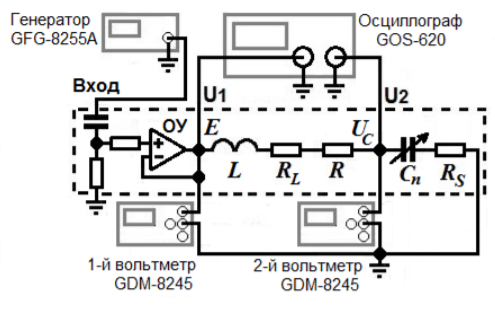
\includegraphics[width = 18cm]{setup.png}
    \caption{Схема экспериментальной цепи}
\end{figure}

\newpage

\section*{Ход работы}

Были сняты данные для амплитудно-частотной и фазо-частотной характеристик для емкостей $C_2 = 33.4$ нФ и $C_5 = 67.4$ нФ. Для АЧХ получился следующий график:

\begin{figure}[h]
    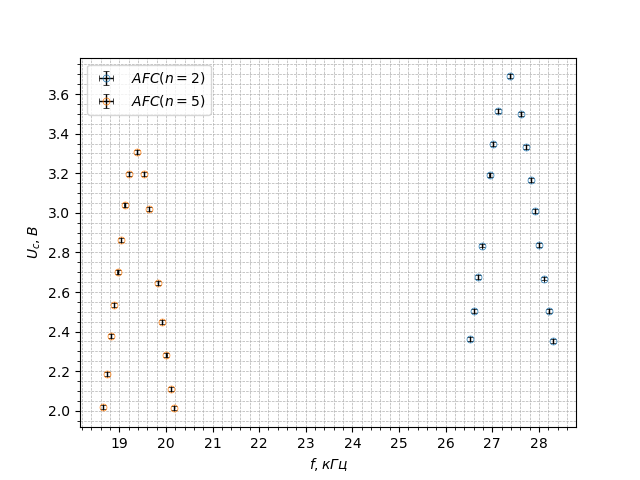
\includegraphics[width = \textwidth]{AFC/graphs/combined_graph.png}
    \caption{АЧХ для емкостей $C_2$ (справа) и $C_5$ (слева)}
\end{figure}

\begin{figure}[H]
	\centering
	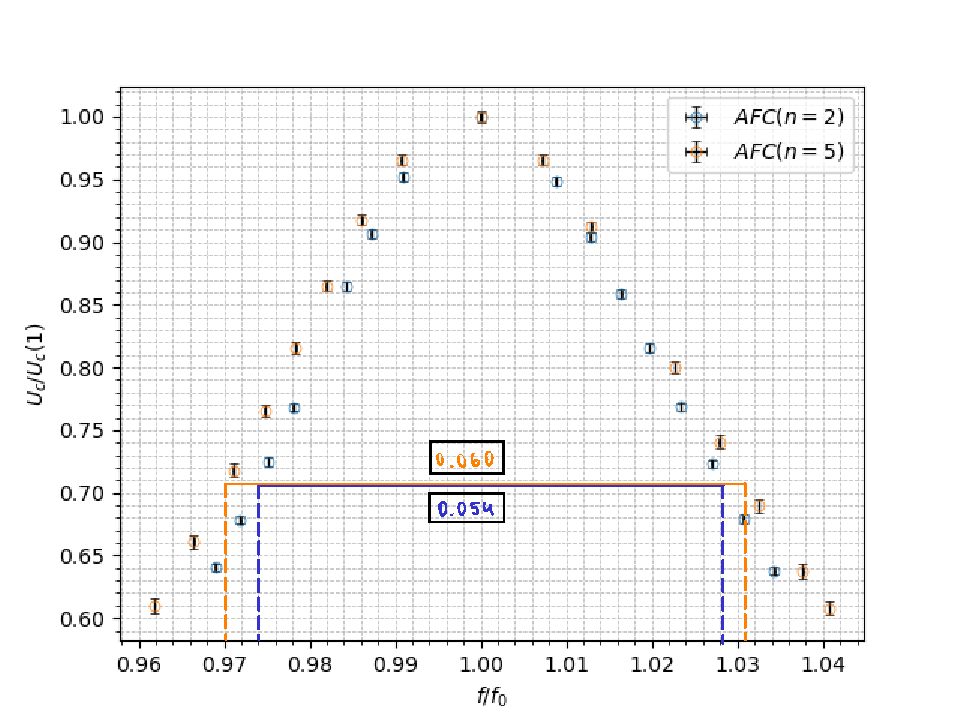
\includegraphics[width = 0.85\textwidth, height = 0.44\textheight]{AFC_dimensionless/graphs/combined_marked.pdf}
	\caption{АЧХ в относительном масштабе}
\end{figure}

Видно, что большей емкости отвечает кривая с большей шириной (так как добротность ниже). Измерим добротности с помощью ширины резонансной кривой на графике в относительном масштабе. Получились следующие значения:

\begin{table}[h]
    \centering
    \begin{tabular}{|c|c|c|c|c|}
        \hline
        $n$ & $C$, нФ & $\frac{2\Delta \nu}{\nu_0}$ & $Q$ & $\sigma_Q$ \\ \hline
        2 & 33.2 & 0.060 & 18.51 & 0.48 \\ \hline
        5 & 67.4 & 0.054 & 16.66 & 0.39 \\ \hline
    \end{tabular}
    \caption{Расчет добротности по ширине АЧХ}
\end{table}

Рассчитаем также добротность по ФЧХ: измерим ширину кривой, которая ограничивается значениями $\frac{\Delta \phi}{\pi}$ от 0,25 до 0,75, получим следующие значения добротностей:

\begin{figure}[H]
    \centering
    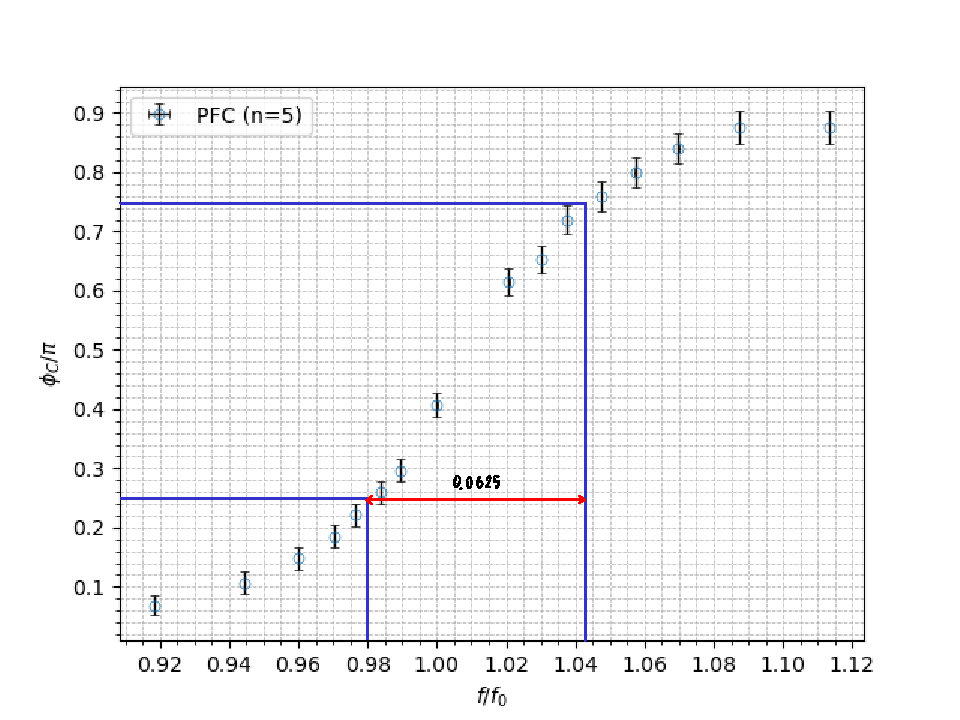
\includegraphics[width = 0.75\textwidth, height = 0.40\textheight]{PFC/graphs/combined_marked.pdf}
    \caption{ФЧХ в относительном масштабе}
\end{figure}

\begin{table}[H]
    \centering
    \begin{tabular}{|c|c|c|c|c|}
        \hline
        $n$ & $C$, нФ & $\frac{2\Delta \nu}{\nu_0}$ & $Q$ & $\sigma_Q$ \\ \hline
        5 & 67.4 & 0.0625 & 16.00 & 1.37  \\ \hline
    \end{tabular}
    \caption{Расчет добротности по ширине ФЧХ}
\end{table}

Построим теперь график зависимость $R_L(\nu)$.

\begin{figure}[H]
    \centering
    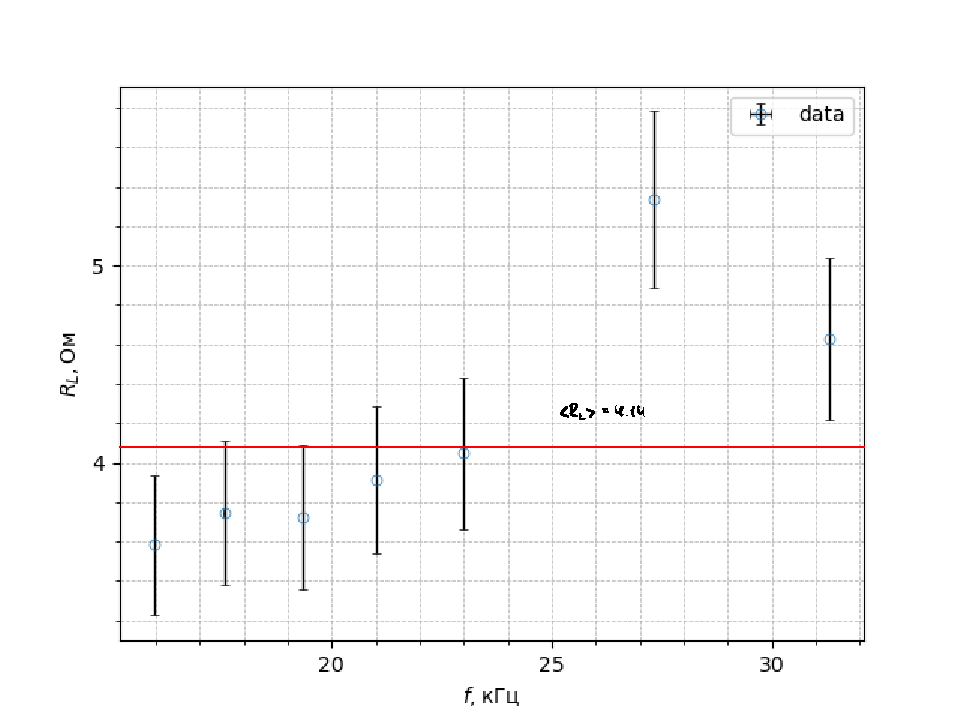
\includegraphics[width = 0.85\textwidth]{R_L-f_0/graphs/marked.pdf}
    \caption{Зависимость $R_L(\nu)$}
\end{figure}


\begin{equation}
    R_L = (4.14 \pm 0.63) \; \text{Ом} \; (\varepsilon = 15 \%)
\end{equation}

Требуется также построить векторные диаграммы токов и напряжений при резонансе для контура с минимальной добротностью. Так как контур последовательный, то токи будут находится на всех элементах в одной фазе. А вот с напряжением ситуация другая: напряжения на конденсаторе и катушке почти в противофазе, причем из напряжение на катушке опережает $\mathcal{E}$ на $\frac{\pi}{2}$, а напряжение на конденсаторе отстаёт от $\mathcal{E}$ на $\frac{\pi}{2}$.
	$U_L$ расположена под углом $\varphi = 88,1$\textdegree, так как на катушке есть еще активное сопротивление $R_L$. $\tg{\varphi}$ можно рассчитать как $\frac{U_{C_{\text{рез}}}}{IR_L}$.

\begin{figure}[H]
    \centering
    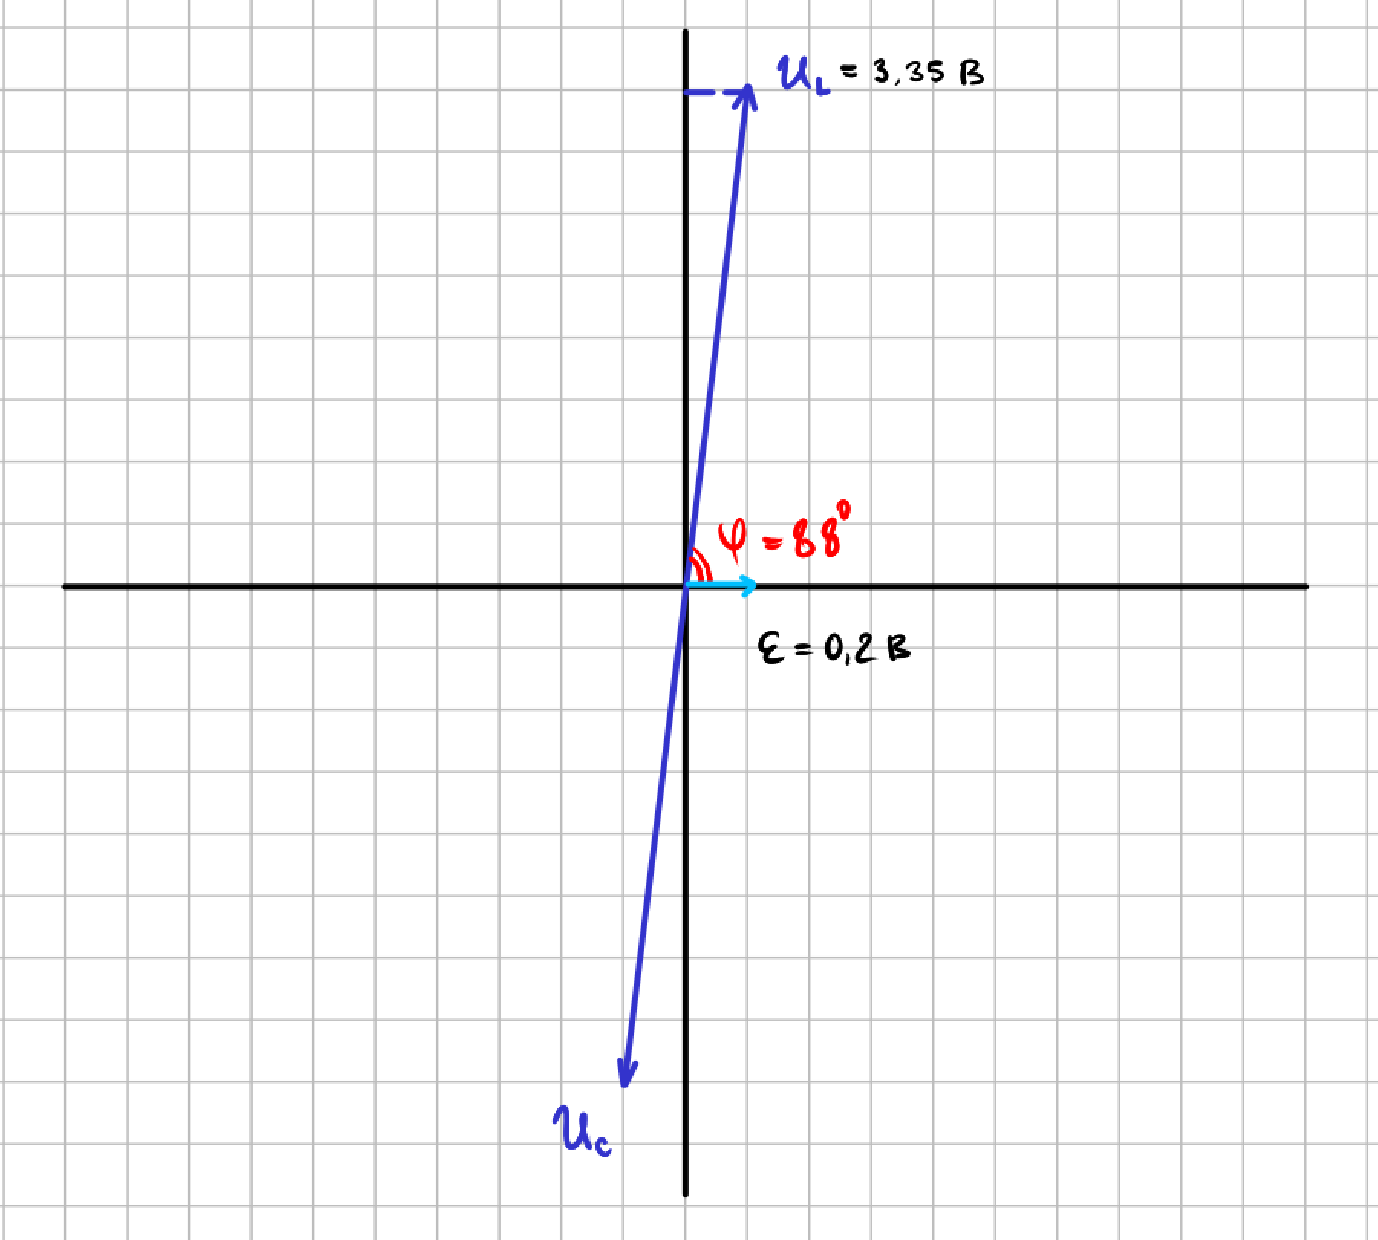
\includegraphics[width = 0.85\textwidth]{vecd.pdf}
    \caption{Векторная диаграмма}
\end{figure}

\section*{Вывод}

Погрешность при расчете добротности через ширину резонансных кривых получилась достаточно большой. Данная неточность может быть объяснена тем, что получившиеся АЧХ и ФЧХ страдают из-за небольшего количество точек, а также из-за некоторой их неравномерности. Тем не менее погрешность добротности в случае АЧХ получилась вполне себе неплохой. В случае ФЧХ мы сначала снимали данные с осциллографа (неточность №1), а потом примерно измерели ширину резонансной кривой (неточность №2). Измерения по параметрам контура точнее.

Можем также заметить, что активное сопротивлени катушки $R_L$ линейно растет с частотой, что обусловлено скин-эффектом. Суть эффекта состоит в вытеснении тока в поверхностные слои провода. Как следствие, уменьшается полезное сечение проводника и растет сопротивление.




\end{document}
